% FIGURE 4: Slack-Safety Region
% Improved aesthetics: Unified color scheme, clear annotations
\begin{figure}[tb]
\centering
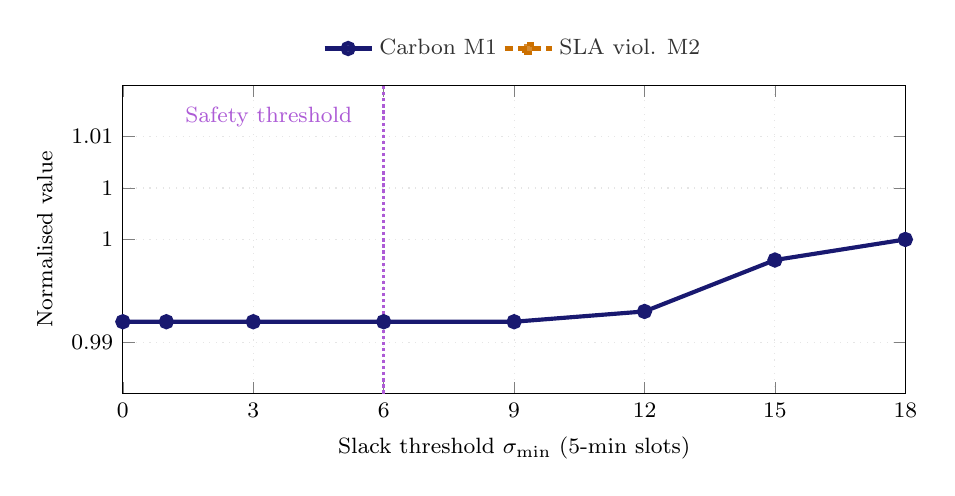
\begin{tikzpicture}
\begin{axis}[
  width=0.95\columnwidth, height=5.5cm,
  xlabel={Slack threshold $\sigma_{\min}$ (5-min slots)},
  ylabel={Normalised value},
  xmin=0, xmax=18, ymin=0.98, ymax=1.01,
  xtick={0,3,6,9,12,15,18},
  ytick={0.985, 0.995, 1.000, 1.005},
  grid=both, grid style={dotted, black!10},
  tick label style={font=\footnotesize}, label style={font=\footnotesize},
  legend style={font=\footnotesize, draw=none, fill=white, fill opacity=0.8,
    legend columns=-1, at={(0.5,1.05)}, anchor=south},
  every axis plot/.append style={line width=1.5pt}
]
% Carbon (M1) 
\addplot[MidnightBlue, mark=*, mark size=2pt] coordinates {
 (0,0.987)(1,0.987)(3,0.987)(6,0.987)(9,0.987)(12,0.988)(15,0.993)(18,0.995)
};
\addlegendentry{Carbon M1}
% SLA violation (M2)
\addplot[DarkOrange!80!black, densely dashed, mark=square*, mark size=1.5pt] coordinates {
 (0,0.000)(1,0.000)(3,0.000)(6,0.000)(9,0.000)(12,0.000)(15,0.000)(18,0.000)
};
\addlegendentry{SLA viol. M2}
% Safety boundary annotation
\draw[densely dotted, line width=1.2pt, DarkOrchid!80] (axis cs:6,0.98) -- (axis cs:6,1.01);
\node[font=\footnotesize, text=DarkOrchid!80, anchor=south east] at (axis cs:5.5,1.005) {Safety threshold};
\end{axis}
\end{tikzpicture}
\caption{Slack-safety region (real Azure Functions 2019 trace,
Theorem~\ref{thm:slack}). The SLA violation rate (M2, dashed) stays
at zero for all $\sigma_{\min}$ values. Carbon M1 (solid) degrades
slightly as the threshold tightens, since fewer jobs can be deferred
safely. The operator selects $\sigma_{\min}=6$ (dotted line) as a
practical safety knob.}
\label{fig:slack}
\end{figure}
